% Options for packages loaded elsewhere
\PassOptionsToPackage{unicode}{hyperref}
\PassOptionsToPackage{hyphens}{url}
%
\documentclass[
  english,
  man]{apa6}
\usepackage{lmodern}
\usepackage{amssymb,amsmath}
\usepackage{ifxetex,ifluatex}
\ifnum 0\ifxetex 1\fi\ifluatex 1\fi=0 % if pdftex
  \usepackage[T1]{fontenc}
  \usepackage[utf8]{inputenc}
  \usepackage{textcomp} % provide euro and other symbols
\else % if luatex or xetex
  \usepackage{unicode-math}
  \defaultfontfeatures{Scale=MatchLowercase}
  \defaultfontfeatures[\rmfamily]{Ligatures=TeX,Scale=1}
\fi
% Use upquote if available, for straight quotes in verbatim environments
\IfFileExists{upquote.sty}{\usepackage{upquote}}{}
\IfFileExists{microtype.sty}{% use microtype if available
  \usepackage[]{microtype}
  \UseMicrotypeSet[protrusion]{basicmath} % disable protrusion for tt fonts
}{}
\makeatletter
\@ifundefined{KOMAClassName}{% if non-KOMA class
  \IfFileExists{parskip.sty}{%
    \usepackage{parskip}
  }{% else
    \setlength{\parindent}{0pt}
    \setlength{\parskip}{6pt plus 2pt minus 1pt}}
}{% if KOMA class
  \KOMAoptions{parskip=half}}
\makeatother
\usepackage{xcolor}
\IfFileExists{xurl.sty}{\usepackage{xurl}}{} % add URL line breaks if available
\IfFileExists{bookmark.sty}{\usepackage{bookmark}}{\usepackage{hyperref}}
\hypersetup{
  pdftitle={Sexism and Division of Labor on Feelings of Teamliness Within Household Dyads},
  pdfauthor={Naomi Liftman1 \& Cara Krupnikoff-Salkin1},
  pdflang={en-EN},
  pdfkeywords={keywords},
  hidelinks,
  pdfcreator={LaTeX via pandoc}}
\urlstyle{same} % disable monospaced font for URLs
\usepackage{graphicx,grffile}
\makeatletter
\def\maxwidth{\ifdim\Gin@nat@width>\linewidth\linewidth\else\Gin@nat@width\fi}
\def\maxheight{\ifdim\Gin@nat@height>\textheight\textheight\else\Gin@nat@height\fi}
\makeatother
% Scale images if necessary, so that they will not overflow the page
% margins by default, and it is still possible to overwrite the defaults
% using explicit options in \includegraphics[width, height, ...]{}
\setkeys{Gin}{width=\maxwidth,height=\maxheight,keepaspectratio}
% Set default figure placement to htbp
\makeatletter
\def\fps@figure{htbp}
\makeatother
\setlength{\emergencystretch}{3em} % prevent overfull lines
\providecommand{\tightlist}{%
  \setlength{\itemsep}{0pt}\setlength{\parskip}{0pt}}
\setcounter{secnumdepth}{-\maxdimen} % remove section numbering
% Make \paragraph and \subparagraph free-standing
\ifx\paragraph\undefined\else
  \let\oldparagraph\paragraph
  \renewcommand{\paragraph}[1]{\oldparagraph{#1}\mbox{}}
\fi
\ifx\subparagraph\undefined\else
  \let\oldsubparagraph\subparagraph
  \renewcommand{\subparagraph}[1]{\oldsubparagraph{#1}\mbox{}}
\fi
% Manuscript styling
\usepackage{upgreek}
\captionsetup{font=singlespacing,justification=justified}

% Table formatting
\usepackage{longtable}
\usepackage{lscape}
% \usepackage[counterclockwise]{rotating}   % Landscape page setup for large tables
\usepackage{multirow}		% Table styling
\usepackage{tabularx}		% Control Column width
\usepackage[flushleft]{threeparttable}	% Allows for three part tables with a specified notes section
\usepackage{threeparttablex}            % Lets threeparttable work with longtable

% Create new environments so endfloat can handle them
% \newenvironment{ltable}
%   {\begin{landscape}\centering\begin{threeparttable}}
%   {\end{threeparttable}\end{landscape}}
\newenvironment{lltable}{\begin{landscape}\centering\begin{ThreePartTable}}{\end{ThreePartTable}\end{landscape}}

% Enables adjusting longtable caption width to table width
% Solution found at http://golatex.de/longtable-mit-caption-so-breit-wie-die-tabelle-t15767.html
\makeatletter
\newcommand\LastLTentrywidth{1em}
\newlength\longtablewidth
\setlength{\longtablewidth}{1in}
\newcommand{\getlongtablewidth}{\begingroup \ifcsname LT@\roman{LT@tables}\endcsname \global\longtablewidth=0pt \renewcommand{\LT@entry}[2]{\global\advance\longtablewidth by ##2\relax\gdef\LastLTentrywidth{##2}}\@nameuse{LT@\roman{LT@tables}} \fi \endgroup}

% \setlength{\parindent}{0.5in}
% \setlength{\parskip}{0pt plus 0pt minus 0pt}

% \usepackage{etoolbox}
\makeatletter
\patchcmd{\HyOrg@maketitle}
  {\section{\normalfont\normalsize\abstractname}}
  {\section*{\normalfont\normalsize\abstractname}}
  {}{\typeout{Failed to patch abstract.}}
\patchcmd{\HyOrg@maketitle}
  {\section{\protect\normalfont{\@title}}}
  {\section*{\protect\normalfont{\@title}}}
  {}{\typeout{Failed to patch title.}}
\makeatother
\shorttitle{Sexism and Feelings of Teamliness}
\keywords{keywords\newline\indent Word count: X}
\DeclareDelayedFloatFlavor{ThreePartTable}{table}
\DeclareDelayedFloatFlavor{lltable}{table}
\DeclareDelayedFloatFlavor*{longtable}{table}
\makeatletter
\renewcommand{\efloat@iwrite}[1]{\immediate\expandafter\protected@write\csname efloat@post#1\endcsname{}}
\makeatother
\usepackage{csquotes}
\ifxetex
  % Load polyglossia as late as possible: uses bidi with RTL langages (e.g. Hebrew, Arabic)
  \usepackage{polyglossia}
  \setmainlanguage[]{english}
\else
  \usepackage[shorthands=off,main=english]{babel}
\fi

\title{Sexism and Division of Labor on Feelings of Teamliness Within Household Dyads}
\author{Naomi Liftman\textsuperscript{1} \& Cara Krupnikoff-Salkin\textsuperscript{1}}
\date{}


\affiliation{\vspace{0.5cm}\textsuperscript{1} Smith College}

\begin{document}
\maketitle

\hypertarget{methods}{%
\section{Methods}\label{methods}}

\hypertarget{measures}{%
\subsection{Measures}\label{measures}}

\hypertarget{independent-variables}{%
\subsubsection{Independent Variables}\label{independent-variables}}

Hostile sexism (HS) and benevolent sexism (BS) were measured using a modified version of the Ambivalent Sexism Inventory (ASI) created by Glick and Fiske (1997). The original scale includes 22 questions with 11 for both subcategories of sexism; however, we removed question 18, \enquote{There are actually very few women who get a kick out of teasing men by seeming sexually available and then refusing male advances}. Participants did not appear to understand the wording of the question, and responses were inconsistent with their other answers. Therefore, our final data includes 10 questions assessing HS and 11 assessing BS. A higher score for either scale indicates higher sexist beliefs. Alphas for HS and BS were .87 and .80 respectively and the intraclass correlations were .59 and .32.

To calculate the division of household labor we asked each participant to complete 14 daily diaries, in which they were given a list of routine chores and were asked to indicate, \enquote{Today, did you spend any time on the following household chores?} Since we are looking to isolate routine chores, we chose to omit intermittent chores from our calculation of housework. We removed the responses to the categories \enquote{Took care of our cars today (sent to repairs, washing, vacuuming)} and \enquote{Prepared for events and activities today (for example, birthdays or anniversaries)}. We also chose not to include text responses of additional chores because most of them fell into other chore categories or were better described as intermittent. There were 11 remaining chores (e.g., laundry, cooking, yardwork, etc.) and the intraclass correlation was .38.

\hypertarget{response-variable}{%
\subsubsection{Response Variable}\label{response-variable}}

In order to assess feelings about working together as partners, participants were asked about the degree to which they identified with the statement: \enquote{Today, my partner and I are really a team} in their daily diaries. Their answers were scored on a four point scale, with possible responses ranging from \emph{mostly true about me} to \emph{not true about me}. A higher score was associated with lower feelings about the quality of teamwork for the day. The intraclass correlation for this variable was -0.91.

\hypertarget{participants}{%
\subsection{Participants}\label{participants}}

While the original data set includes 364 participants of all identities, it predominantly consists of heterosexual individuals (\emph{n} = 353). In order to examine division of labor along gender lines, it was necessary to restrict the data set to male-female couples. Due to the small number of male-female couples that included an individual who was not heterosexual, we decided to restrict our sample further to only include heterosexual couples. This was done in order to prevent any confounds that sexual orientation may have caused. Additionally, since all of the couples were living together, we included both couples who were married and those who were in long-term relationships. Regardless of marital status, couples who have lived together for some time need to find ways to divide their housework, and are therefore relevant to our study.

After cleaning the data and filtering out any missing or problematic data points, we were left with 272 individuals (136 dyads). Of the participants, there were 127 married couples, 7 couples that were in committed, long-term relationships and 2 couples where one individual answered that they were married and the other answered that they were in a long-term relationship. All 136 of the couples answered that they were living together. Notably, 50 participants didn't answer any of the demographic information. In these cases, the partner's information was used in calculating these numbers. When looking at other household members, 45 of the couples had children under the age of 18 living in their homes. 36 had one child, 31 had two, 13 had three, and 5 had four. Additionally, one couple reported having ten children, and another reported having 26. These two cases may have been participant error when they were inputting the amount of children in their households as text answers. Five couples had one individual report a different number of children than the other. Those who did not answer the question were coded as having no children.

A majority of the participants were White (\emph{n} = 165). 24 participants identified as Asian, 17 identified as Black or African American, 9 identified as Hispanic or Latinx, 2 as Middle Eastern, 3 as White and Hispanic/Latinx, and 52 either did not answer or chose the \enquote{prefer not to answer} option. 9 of the couples were mixed-race couples. A majority of the individuals identified themselves as Christian (\emph{n} = 150). A wide assortment of other religions were also represented, but none had more than 15 people affiliated with them. In terms of political affiliations, there was a pretty equal distribution along the spectrum. Most of the individuals were at or around the center of the spectrum, with a slight skew towards conservatism.

\begin{verbatim}
## # A tibble: 2 x 4
##   gender2_A     n     m    sd
##   <chr>     <int> <dbl> <dbl>
## 1 Man          21  3.56 0.811
## 2 Woman        22  3.23 1.01
\end{verbatim}

\begin{verbatim}
## # A tibble: 2 x 4
##   gender2_A     n     m    sd
##   <chr>     <int> <dbl> <dbl>
## 1 Man          21  3.95 0.696
## 2 Woman        22  3.71 0.716
\end{verbatim}

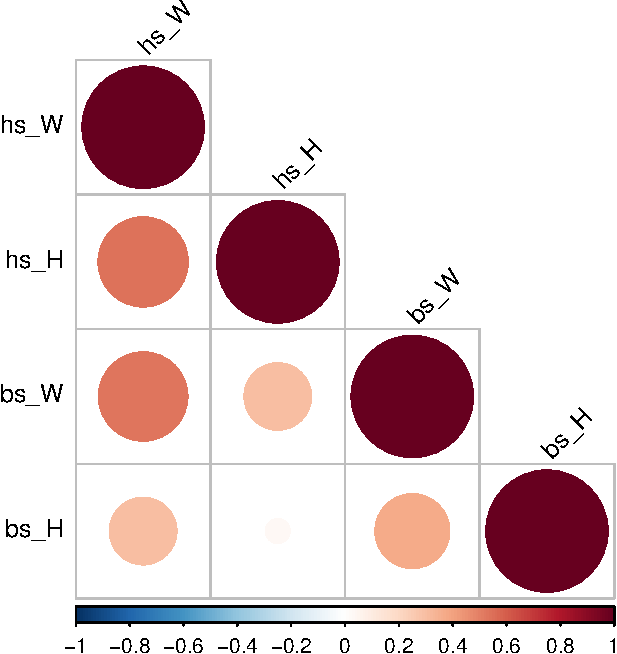
\includegraphics{Final_Paper_files/figure-latex/table-1.pdf}

\begin{verbatim}
##      hs_W  hs_H bs_W bs_H
## hs_W    1                
## hs_H 0.54     1          
## bs_W 0.53   0.3    1     
## bs_H  0.3 0.038 0.37    1
\end{verbatim}

\begin{verbatim}
##         hs_W   hs_H    bs_W bs_H
## hs_W       0                    
## hs_H 8.1e-08      0             
## bs_W 9.4e-05 0.0044       0     
## bs_H  0.0046   0.81 0.00056    0
\end{verbatim}

\begin{table}

\caption{\label{tab:unnamed-chunk-2}Table 1. Correlation Matrix Between Sexism Scores}
\begin{tabular}[t]{l|r|r|l|l|l|l}
\hline
\multicolumn{3}{c|}{ } & \multicolumn{4}{c}{Correlations} \\
\cline{4-7}
Scales & Mean & SD & X1 & X2 & X3 & X4\\
\hline
1X Male Hostile Sexism & 3.56 & 0.810 & 1 & .038 & .54 & .3\\
\hline
2X Male Benevolent Sexism & 3.95 & 0.696 & .038 & 1 & .3 & .37\\
\hline
3X Female Hostile Sexism & 3.23 & 1.010 & .54 & .3 & 1 & .53\\
\hline
4X Female Benevolent Sexism & 3.71 & 0.720 & .3 & .37 & .53 & 1\\
\hline
\multicolumn{7}{l}{\rule{0pt}{1em}\textit{Note: }}\\
\multicolumn{7}{l}{\rule{0pt}{1em}Possible scores for hostile and benevolent sexism ranged from 1 to 7. All correlations except for male hostile sexism with male benevolent sexism was statistically signficinat with p < .01}\\
\end{tabular}
\end{table}

\hypertarget{data-analysis}{%
\subsection{Data analysis}\label{data-analysis}}

We used R (Version 4.1.1; R Core Team, 2022) and the R-packages \emph{dplyr} (Version 1.0.8; Wickham et al., 2022a), \emph{forcats} (Version 0.5.1; Wickham, 2021), \emph{ggformula} (Version 0.10.1; Kaplan \& Pruim, 2021), \emph{ggplot2} (Version 3.3.5; Wickham, 2016), \emph{ggridges} (Version 0.5.3; Wilke, 2021), \emph{ggstance} (Version 0.3.5; Henry et al., 2020), \emph{gtable} (Version 0.3.0; Wickham \& Pedersen, 2019), \emph{kableExtra} (Version 1.3.4; Zhu, 2021), \emph{lattice} (Version 0.20.44; Sarkar, 2008), \emph{lubridate} (Version 1.7.10; Grolemund \& Wickham, 2011), \emph{Matrix} (Version 1.3.4; Bates \& Maechler, 2021), \emph{mosaic} (Version 1.8.3; Pruim, Kaplan, \& Horton, 2017, 2021), \emph{mosaicData} (Version 0.20.2; Pruim et al., 2021), \emph{nlme} (Version 3.1.153; Pinheiro, Bates, DebRoy, Sarkar, \& R Core Team, 2022), \emph{papaja} (Version 0.1.0.9997; Aust \& Barth, 2020), \emph{psych} (Version 2.1.9; Revelle, 2021), \emph{purrr} (Version 0.3.4; Henry \& Wickham, 2020), \emph{readr} (Version 2.0.1; Wickham et al., 2022b), \emph{stringr} (Version 1.4.0; Wickham, 2019), \emph{tibble} (Version 3.1.6; Müller \& Wickham, 2021), \emph{tidyr} (Version 1.1.3; Wickham \& Girlich, 2022), and \emph{tidyverse} (Version 1.3.1; Wickham, Averick, et al., 2019) for all our analyses.

\newpage

\hypertarget{references}{%
\section{References}\label{references}}

\begingroup
\setlength{\parindent}{-0.5in}
\setlength{\leftskip}{0.5in}

\hypertarget{refs}{}
\leavevmode\hypertarget{ref-R-papaja}{}%
Aust, F., \& Barth, M. (2020). \emph{papaja: Create APA manuscripts with R Markdown}. Retrieved from \url{https://github.com/crsh/papaja}

\leavevmode\hypertarget{ref-R-Matrix}{}%
Bates, D., \& Maechler, M. (2021). \emph{Matrix: Sparse and dense matrix classes and methods}. Retrieved from \url{https://CRAN.R-project.org/package=Matrix}

\leavevmode\hypertarget{ref-ASI}{}%
Glick, P., \& Fiske, S. (1997). \emph{Psychology of Women Quarterly}, \emph{21}(1), 119--135. \url{https://doi.org/10.1111/j.1471-6402.1997.tb00104.x}

\leavevmode\hypertarget{ref-R-lubridate}{}%
Grolemund, G., \& Wickham, H. (2011). Dates and times made easy with lubridate. \emph{Journal of Statistical Software}, \emph{40}(3), 1--25. Retrieved from \url{https://www.jstatsoft.org/v40/i03/}

\leavevmode\hypertarget{ref-R-purrr}{}%
Henry, L., \& Wickham, H. (2020). \emph{Purrr: Functional programming tools}. Retrieved from \url{https://CRAN.R-project.org/package=purrr}

\leavevmode\hypertarget{ref-R-ggstance}{}%
Henry, L., Wickham, H., \& Chang, W. (2020). \emph{Ggstance: Horizontal 'ggplot2' components}. Retrieved from \url{https://CRAN.R-project.org/package=ggstance}

\leavevmode\hypertarget{ref-R-ggformula}{}%
Kaplan, D., \& Pruim, R. (2021). \emph{Ggformula: Formula interface to the grammar of graphics}. Retrieved from \url{https://CRAN.R-project.org/package=ggformula}

\leavevmode\hypertarget{ref-R-tibble}{}%
Müller, K., \& Wickham, H. (2021). \emph{Tibble: Simple data frames}. Retrieved from \url{https://CRAN.R-project.org/package=tibble}

\leavevmode\hypertarget{ref-R-nlme}{}%
Pinheiro, J., Bates, D., DebRoy, S., Sarkar, D., \& R Core Team. (2022). \emph{nlme: Linear and nonlinear mixed effects models}. Retrieved from \url{https://CRAN.R-project.org/package=nlme}

\leavevmode\hypertarget{ref-R-mosaicData}{}%
Pruim, R., Kaplan, D., \& Horton, N. (2021). \emph{MosaicData: Project mosaic data sets}. Retrieved from \url{https://CRAN.R-project.org/package=mosaicData}

\leavevmode\hypertarget{ref-R-mosaic}{}%
Pruim, R., Kaplan, D. T., \& Horton, N. J. (2017). The mosaic package: Helping students to 'think with data' using r. \emph{The R Journal}, \emph{9}(1), 77--102. Retrieved from \url{https://journal.r-project.org/archive/2017/RJ-2017-024/index.html}

\leavevmode\hypertarget{ref-R-base}{}%
R Core Team. (2022). \emph{R: A language and environment for statistical computing}. Vienna, Austria: R Foundation for Statistical Computing. Retrieved from \url{https://www.R-project.org/}

\leavevmode\hypertarget{ref-R-psych}{}%
Revelle, W. (2021). \emph{Psych: Procedures for psychological, psychometric, and personality research}. Evanston, Illinois: Northwestern University. Retrieved from \url{https://CRAN.R-project.org/package=psych}

\leavevmode\hypertarget{ref-R-lattice}{}%
Sarkar, D. (2008). \emph{Lattice: Multivariate data visualization with r}. New York: Springer. Retrieved from \url{http://lmdvr.r-forge.r-project.org}

\leavevmode\hypertarget{ref-R-ggplot2}{}%
Wickham, H. (2016). \emph{Ggplot2: Elegant graphics for data analysis}. Springer-Verlag New York. Retrieved from \url{https://ggplot2.tidyverse.org}

\leavevmode\hypertarget{ref-R-stringr}{}%
Wickham, H. (2019). \emph{Stringr: Simple, consistent wrappers for common string operations}. Retrieved from \url{https://CRAN.R-project.org/package=stringr}

\leavevmode\hypertarget{ref-R-forcats}{}%
Wickham, H. (2021). \emph{Forcats: Tools for working with categorical variables (factors)}. Retrieved from \url{https://CRAN.R-project.org/package=forcats}

\leavevmode\hypertarget{ref-R-tidyverse}{}%
Wickham, H., Averick, M., Bryan, J., Chang, W., McGowan, L. D., François, R., \ldots{} Yutani, H. (2019). Welcome to the tidyverse. \emph{Journal of Open Source Software}, \emph{4}(43), 1686. \url{https://doi.org/10.21105/joss.01686}

\leavevmode\hypertarget{ref-R-dplyr}{}%
Wickham, H., François, R., Henry, L., \& Müller, K. (2022a). \emph{Dplyr: A grammar of data manipulation}. Retrieved from \url{https://CRAN.R-project.org/package=dplyr}

\leavevmode\hypertarget{ref-R-tidyr}{}%
Wickham, H., \& Girlich, M. (2022). \emph{Tidyr: Tidy messy data}. Retrieved from \url{https://CRAN.R-project.org/package=tidyr}

\leavevmode\hypertarget{ref-R-readr}{}%
Wickham, H., Hester, J., \& Bryan, J. (2022b). \emph{Readr: Read rectangular text data}. Retrieved from \url{https://CRAN.R-project.org/package=readr}

\leavevmode\hypertarget{ref-R-gtable}{}%
Wickham, H., \& Pedersen, T. L. (2019). \emph{Gtable: Arrange 'grobs' in tables}. Retrieved from \url{https://CRAN.R-project.org/package=gtable}

\leavevmode\hypertarget{ref-R-ggridges}{}%
Wilke, C. O. (2021). \emph{Ggridges: Ridgeline plots in 'ggplot2'}. Retrieved from \url{https://CRAN.R-project.org/package=ggridges}

\leavevmode\hypertarget{ref-R-kableExtra}{}%
Zhu, H. (2021). \emph{KableExtra: Construct complex table with 'kable' and pipe syntax}. Retrieved from \url{https://CRAN.R-project.org/package=kableExtra}

\endgroup


\end{document}
